\documentclass[justified]{tufte-handout}

%\geometry{showframe}% for debugging purposes -- displays the margins

\usepackage{amsmath}

% Set up the images/graphics package
\usepackage{graphicx}
\setkeys{Gin}{width=\linewidth,totalheight=\textheight,keepaspectratio}
\graphicspath{{graphics/}}

\title{Interactive systems for code and data demography}
\author[Elena L. Glassman]{Elena L. Glassman}
%\date{24 January 2009}  % if the \date{} command is left out, the current date will be used

% The following package makes prettier tables.  We're all about the bling!
\usepackage{booktabs}

% The units package provides nice, non-stacked fractions and better spacing
% for units.
\usepackage{units}

\usepackage{xcolor}

% The fancyvrb package lets us customize the formatting of verbatim
% environments.  We use a slightly smaller font.
\usepackage{fancyvrb}
\fvset{fontsize=\normalsize}

% Small sections of multiple columns
\usepackage{multicol}

% Provides paragraphs of dummy text
\usepackage{lipsum}

% These commands are used to pretty-print LaTeX commands
\newcommand{\doccmd}[1]{\texttt{\textbackslash#1}}% command name -- adds backslash automatically
\newcommand{\docopt}[1]{\ensuremath{\langle}\textrm{\textit{#1}}\ensuremath{\rangle}}% optional command argument
\newcommand{\docarg}[1]{\textrm{\textit{#1}}}% (required) command argument
\newenvironment{docspec}{\begin{quote}\noindent}{\end{quote}}% command specification environment
\newcommand{\docenv}[1]{\textsf{#1}}% environment name
\newcommand{\docpkg}[1]{\texttt{#1}}% package name
\newcommand{\doccls}[1]{\texttt{#1}}% document class name
\newcommand{\docclsopt}[1]{\texttt{#1}}% document class option name

\begin{document}

\fontsize{9pt}{12pt}\selectfont

\maketitle% this prints the handout title, author, and date

\begin{marginfigure}%
  \centering
  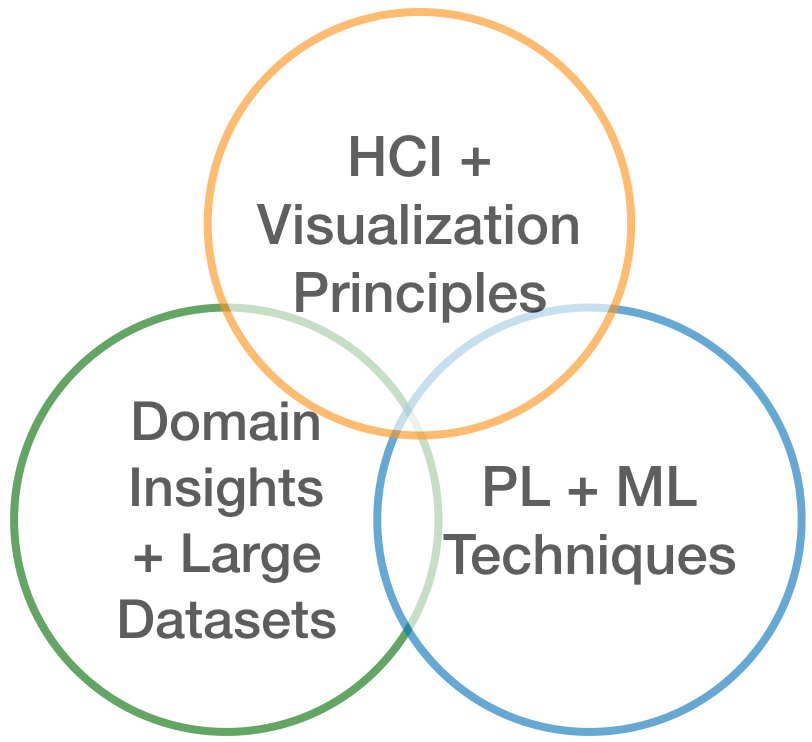
\includegraphics[width=\linewidth]{Summary_figure1.png}
  \caption{Common system components.}
  \label{fig:summaryfig1}
  %\centering
  %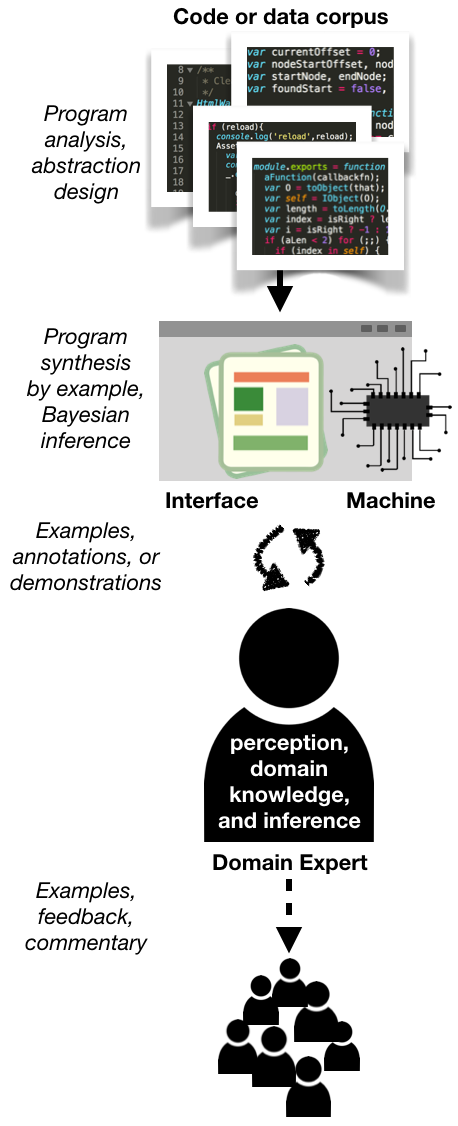
\includegraphics[width=0.75\linewidth]{Summary_figure2.png}
  %\caption{Common system architecture.}
  %\label{fig:summaryfig2}
\end{marginfigure}

%\begin{abstract}
%As an human-computer interaction (HCI) researcher working closely with researchers in programming languages, machine learning, and information theory,
%I design, build and evaluate systems for code and data demography, i.e., comprehending and interacting with population-level structure and trends in large code and data corpora. These systems augment human intelligence by giving users a ``useful degree of comprehension in a situation that previously was too complex.''\cite{engelbart1962} \textcolor{blue}{what's innovative about what I'm doing?}
%\end{abstract}
\begin{abstract}
I use program analysis and synthesis techniques, interactive inference algorithms, visualization principles, and theories from cognitive science to build systems that allow people to (a) complete existing large-scale code and data-related tasks more quickly and (b) answer new questions that were previously prohibitively cognitively demanding or time-consuming to investigate (Fig.~\ref{fig:summaryfig1}). % and~\ref{fig:summaryfig2}
\end{abstract}
%For example, \smallcaps{Overcode} (Fig.~\ref{fig:overcode}) is now deployed at UC Berkeley, where teachers give code composition feedback to more than 1500 students in a few hours.\cite{overcode} 
As an human-computer interaction (HCI) researcher working closely with researchers in programming languages, machine learning, and information theory, I design, build and evaluate systems for code and data demography, i.e., comprehending and interacting with population-level structure and trends in large code and data corpora, and the effects of human-written, synthesized, or learned (ML) programs applied to them. 
%I use the term \emph{demography} is a reference to the population level insights these methods provide at a glance in addition to the preservation of concrete details. 
The systems and interfaces I build augment human intelligence by giving users a ``useful degree of comprehension in a situation that previously was too complex.''\cite{engelbart1962}

The conceptual key to my approach is defining \emph{task-relevant abstractions} using user-centered design or inference algorithms. For example, \smallcaps{Examplore} (Fig.~\ref{fig:examplore}) allows programmers, API designers, and researchers to answer questions about how API methods are actually used in the wild.\cite{examplore} I designed \smallcaps{examplore}'s abstract API skeleton to register and align hundreds of usage examples against each other so that users can get a high-level view of a corpus without sacrificing the ability to read concrete code. This design is supported by theories of human learning, such as analogical learning and Variation Theory: showing multiple aligned examples simultaneously helps induce accurate abstractions in the user's mind. In \smallcaps{FixPropagator}, the abstractions are inferred from expert demonstrations: as a programming teacher begins to fix and give feedback on buggy student code submissions, the back end infers more general, abstract code transformations to propagate fixes and relevant teacher feedback to other buggy student code.\cite{lats17} In our interactive system, the inference is performed by the Microsoft PROgram Synthesis by Example (PROSE) SDK and a custom tree-transforming domain specific language.
\begin{figure*}[h]
  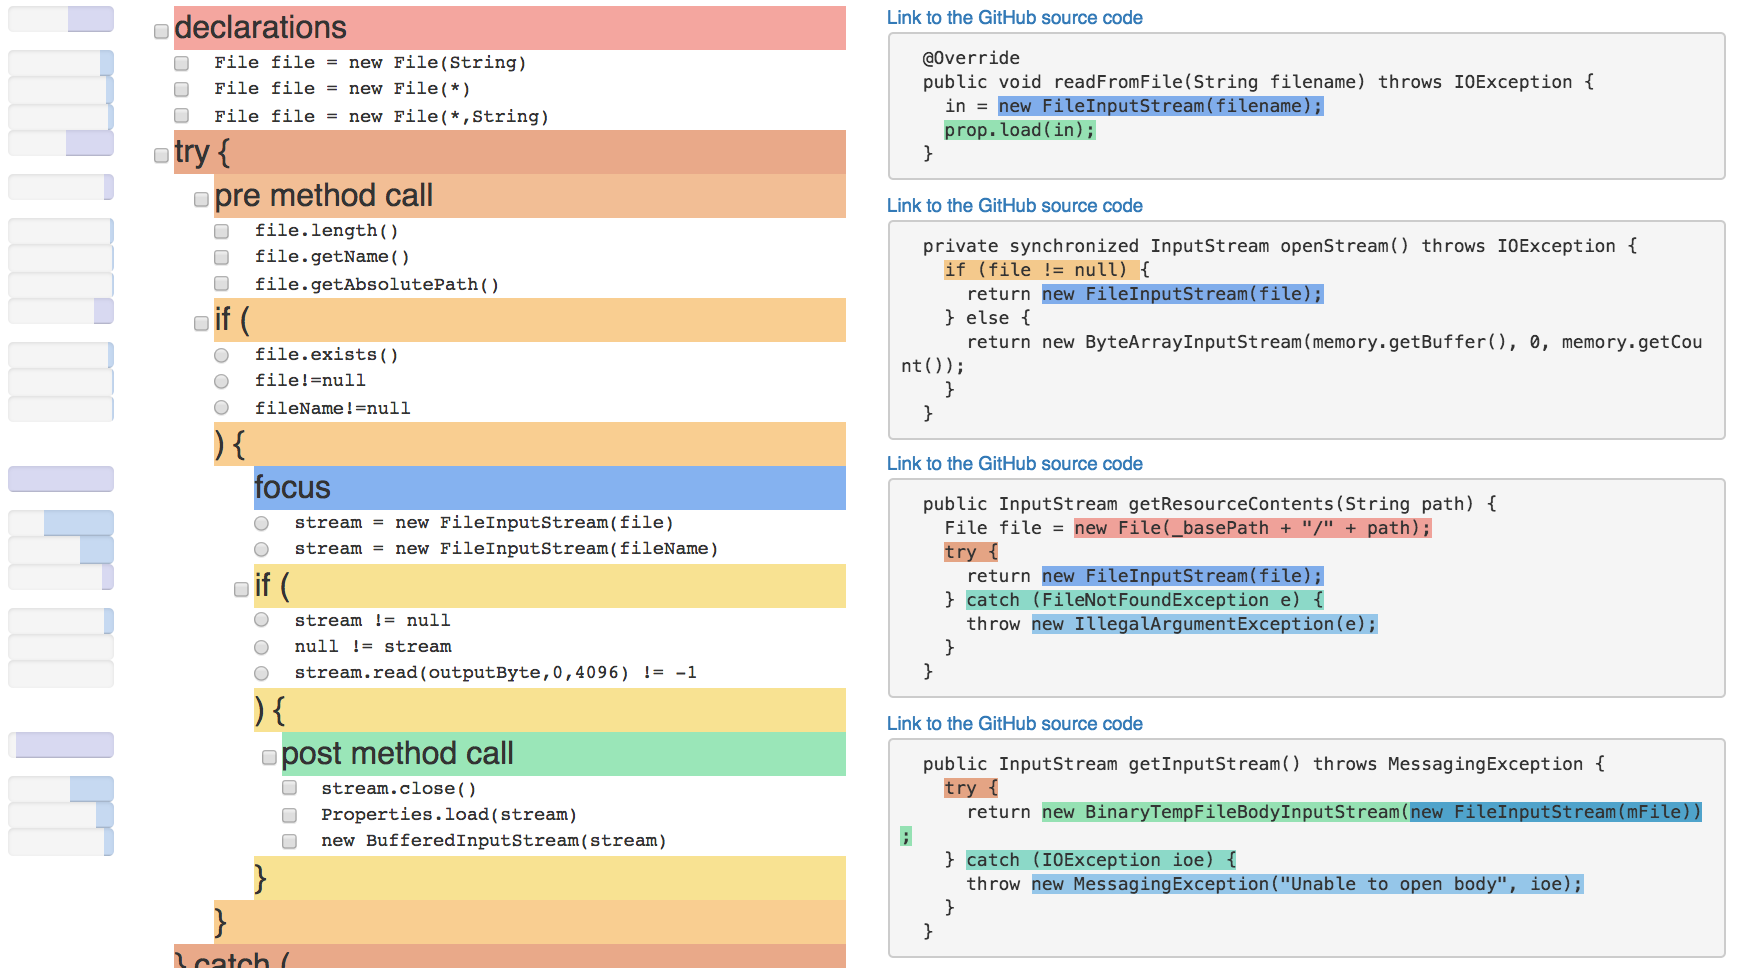
\includegraphics[width=0.64\linewidth]{Statistical_Code_Examples.png}
  \caption{In this screenshot, \smallcaps{Examplore} shows the head of the canonicalized distribution of \texttt{FileInputStream} API usage in 100 open-source Github repositories.}%
  \label{fig:examplore}%
\end{figure*}

\section*{Research directions}

\subsection*{How can we help programmers write better code faster?}

%the team developed a novel code mining and interactive visualization system, EXAMPLORE, that allows users to simultaneously compare and contrast hundreds of API usage examples for a single API, so they can understand the distribution over common and un- common usage patterns of that API in the wild and better answer usage questions. 
%The team calls this approach code demography. 
\smallcaps{examplore} will be the first of a series of tools that transform the modern language, library, and API design, selection, and usage experience for all who program. Björn Hartmann, Miryung Kim, my postdoc Tianyi Zhang, and I are working on new tools for helping programmers (1) how to use APIs in a particular context, (2) how to design and evolve an API, and (3) how to assess an API or select between multiple APIs with similar capabilities.
%In addition to further developing these tools for programmers and library developers in the wild and at companies with large codebases, 
\subsection*{Beyond code}
I am generalizing demography beyond code to help doctors, data scientists, social scientists, journalists, machine learning practitioners, and other end-users comprehend, form hypotheses, act on, and even author programs on large amounts of semi-structured complex data, such as patient records from patients with a common diagnosis, robot trajectories generated for a particular task, and articles on a common topic.\\[0.2cm]
\noindent
\emph{How can we more naturally communicate our intent to machines?}\\
%\subsection{How can humans and machines communicate better about data and the functions applied to them?}
%\textbf{Data-driven human and machine teaching by example}
\noindent
The critical, possibly latent, structural features that distinguish examples from each other help both humans and machines learn concepts and infer abstractions that generalize well. Examples are, therefore, a natural medium for communication between people and machines.
Data demography supports this form of communication: it exposes the population-level characteristics of large datasets in a way that keeps concrete examples front and center instead of hiding them behind nodes in large graphs or other abstractions. I expect that data demography will help users clarify their own intentions\cite{vule} and curate better examples to teach machines, much like \smallcaps{OverCode}\cite{overcode} and \smallcaps{Foobaz}\cite{foobaz} helped teachers understand the state of their massive classroom and pick better examples to address student misconceptions.\\[0.2cm]
%And since the human's and machine's inductive biases when generalizing from examples, interfaces that employ new data demography methods can help humans select the most informative examples with respect to the intent they are trying to communicate to the machine.
\noindent
\emph{How can data demography increase algorithmic transparency?}\\
\noindent
Theories of human concept learning assert that showing people strategically diverse sets of examples will help them construct mental abstractions that generalize well.\cite{vt} When a computer machine-learns or synthesizes a function on a human's behalf, these theories can have implications for which examples are most useful for helping the human construct a useful mental model of the behavior of the otherwise black box function. I plan to build systems that address this challenge by generalizing data demography to reveal \emph{population-level changes} in datasets induced by a function, whether it was human-written, synthesized, or machine-learned.\\[0.2cm] %(The same is true in re when humans teach machines.)
\emph{When the system fails, how do we debug?}\\
\noindent
As powerful as communicating with machines by examples and annotations can be, existing systems can fail in opaque and frustrating ways. How do we build systems that \emph{explain their failure} to synthesize a program that is consistent with user-provided examples? A simple failure mode in program synthesis occurs when the synthesizer's grammar does not match the user's mental model: perhaps the user is teaching the machine how to extract something from raw HTML but the grammar has no notion of matching start and end tags. %The program synthesis toolkit my systems currently use, the Microsoft PROSE SDK, requires an expert-designed grammar to perform well on new tasks and corpora. Rather than co-create abstractions in a fixed grammar, 
What if the machine and the end-user could co-create the grammar itself?
%\section{1. Supporting programmers in the wild and at companies with large codebases}

%Understanding the space of possible code solutions is helpful beyond the classroom, as well. 
%\smallcaps{examplore} (Fig.~\ref{fig:examplore}) is an example of code demography for visualizing and exploring thousands of code examples using the same API: in collaboration with software engineering researchers at UCLA, we created an interactive visualization by mining hundreds of thousands of open-source Github repositories to reveal the common and uncommon ways in which the open-source developer community uses a Java API method.\cite{examplore} To register hundreds of API usage examples against each other for overlaid display, I worked with our collaborators to design an abstraction, the API skeleton, grounded in (1) how API design is taught in their software engineering curricula and (2) how they, as API mining researchers, conceptualize their task. %Interacting with the visualization reveals the facets of the distribution of canonicalized statements and structures enclosing the API method of interest.


%In a lab study, we found that \smallcaps{Examplore} helped programmers understand and answer questions about the distribution of usage patterns of a particular API method in the wild. I hope to make this tool available as an online resource that complements official documentation and Q\&A sites. I also hope to work with companies that have large proprietary codebases and APIs, like Google and Facebook, to customize this tool for their internal on-boarding and code review needs. Through initial contacts, it is clear companies are eager to adopt new tools, like \smallcaps{Examplore}, to increase programmer productivity. 

%\section{1. Tools for teachers and students in massive classrooms}\label{sec:human}

%Enrollment in introductory programming and data science courses is skyrocketing. Even hardware design classes can contain hundreds of students, each constructing their own simulated circuits. %Students have a shared semantic programming goal but they collectively create a large distribution of implementations. It is difficult for teachers to understand what is happening in their classes, and prohibitively labor-intensive to provide expert-level feedback at scale as often as it was possible before enrollments rose dramatically. 
%It is both a challenge and an opportunity to reinvent how we teach students and how students teach each other. With collaborators and mentees, I built, user-tested, and deployed five systems at MIT and UC Berkeley that explore this space of possibilities.%\cite{grovercode}


%see the distribution of student code submissions and misconceptions, discover unusually clever and poor choices, curate sets of examples that clarify important concepts, and give both class-level and automatically personalized individual feedback that can be reused in subsequent semesters. %Two students I mentor are now preparing to make \smallcaps{OverCode} available to all introductory Python programming teachers at any school or university this spring.

%\begin{figure*}[h]
%  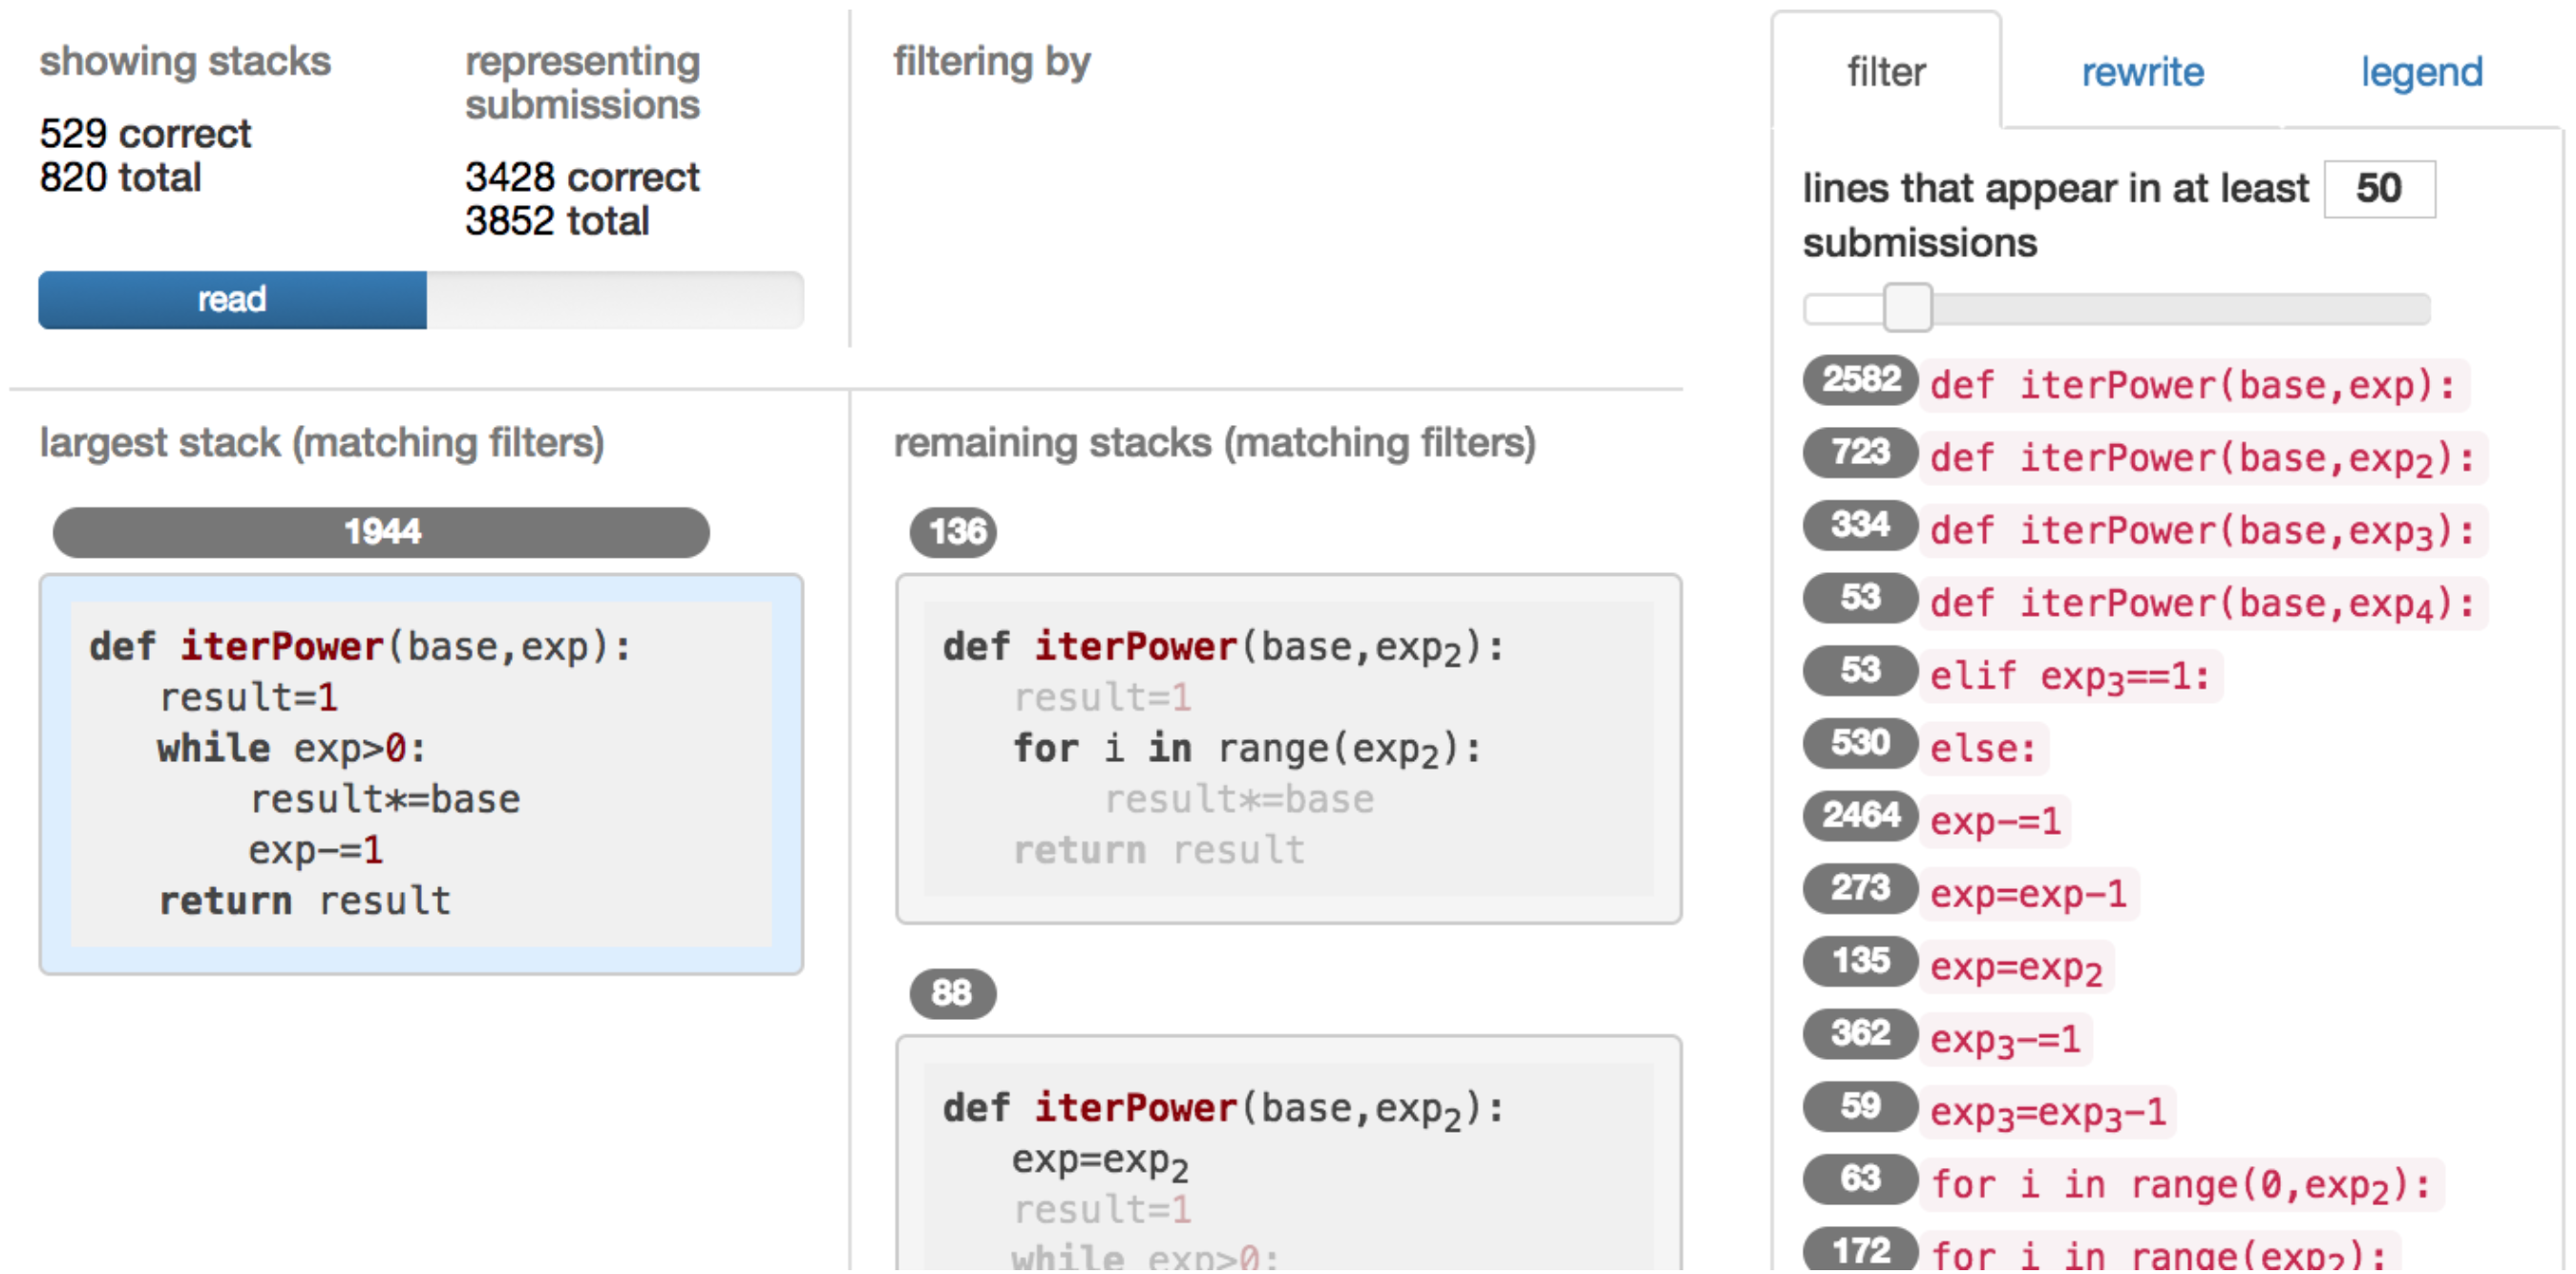
\includegraphics[width=0.65\linewidth]{overcode.png}%
%  \caption{\smallcaps{OverCode} is an example of code demography for teachers in massive programming classes who want to understand the contents of the functions their students wrote.}%
%  \label{fig:overcode}%
%\end{figure*}


%\smallcaps{OverCode} is an example of code demography for visualizing and exploring thousands of solutions to the same programming problem. It uses both static and dynamic analysis to cluster similar solutions and represents each cluster as a synthesized solution that implicitly describes both the cluster center and its boundaries. Teachers can filter and further cluster solutions based on various criteria. One of \smallcaps{OverCode}'s key abstractions is equating variables across solutions based on behavior during execution; these common variables are each renamed to their most popular student-given name, which highlights remaining differences in algorithms and syntax. In user studies, \smallcaps{OverCode} allowed teachers to more quickly develop a high-level view of student understanding and misconceptions, and provide feedback on selected examples that are relevant to more student solutions. %Given its successful integration into programming course infrastructure at UC Berkeley, we hope to make it available to large programming classes at other institutions as well. %A few teachers can give personalized composition feedback on code from over a thousand students in a few hours. The feedback can be automatically reused in following semesters.
%\\\\
%\noindent
%\emph{Societal and potentially commercial impact}\\
%\smallcaps{OverCode} has now been fully integrated into the code composition feedback process of the largest introductory Python programming course at UC Berkeley, which regularly enrolls 1500 students: rather than distributing work to as many as 50 graders, a handful of teaching assistants can give feedback to the entire class in a few hours. We expect that this same feedback will be re-sent to students in future semesters, with little additional effort on the part of the teaching staff. Two Master's students, one at MIT and one at UC Berkeley, have earned---or soon will---their degree in EECS by contributing to this effort and a third student at UC Berkeley is leading the charge to make this tool available to all other schools with large Python programming courses. We are also fielding requests to help others adapt this technology to other programming languages.
%\\\\
%\noindent
%\emph{Scalable, data-driven teaching by example}\\
%Variable names are an important component of code composition, but it is difficult to quickly get an accurate picture of how well all your students are naming variables, and prohibitively time-consuming to comment on individual variable names at scale. \smallcaps{Foobaz} solves this problem by letting teachers draw from their own students' naming choices to create a set of examples that clarify the concept of a good, contextually appropriate variable name.\cite{foobaz} Specifically, \smallcaps{Foobaz} uses \smallcaps{OverCode}'s common variable abstraction to reveal the distribution of student-chosen names for each common variable. Teachers curate and label names of varying quality for the most common variable roles, and \smallcaps{Foobaz} sends each student a set of these examples to evaluate as alternative names for the corresponding variable role in their own program. Students then compare their judgments to teacher labels to help train their inner variable naming critic. %This is a novel, scalable form of data-driven human teaching about code composition.

%\newpage
%\noindent
%\emph{Additional systems}\\
%I also developed and deployed \smallcaps{Dear Beta} and \smallcaps{Dear Gamma} in MIT's large introductory computer architecture course for collecting and distributing student-written debugging and optimization hints for the entire spectrum of student-constructed digital circuits.\cite{cscw16} In the same class, I deployed \smallcaps{Mudslide}, the system I developed at Microsoft Research for collecting and visualizing the distribution and content of student confusion across the slides of a presentation \emph{(CHI Honorable Mention)}.\cite{mudslide} I also supervised an MIT EECS M.Eng. student who created and deployed \smallcaps{GroverCode}, an extension of \smallcaps{overcode} for more quick and consistent exam grading for one of MIT's large introductory Python programming classes.\cite{grovercode}

% \begin{marginfigure}
%   \centering
%   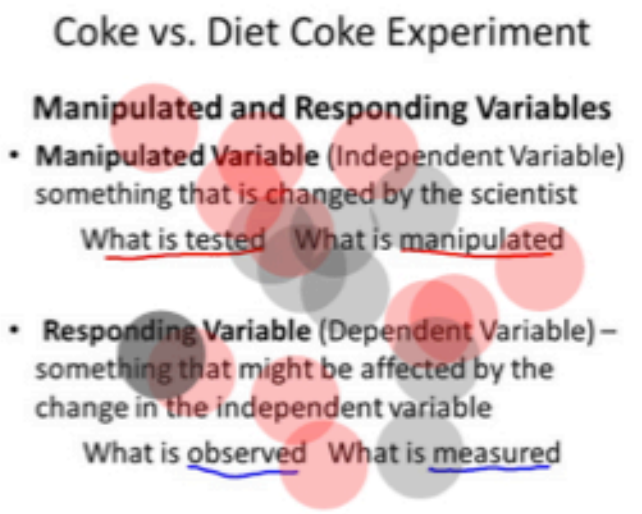
\includegraphics[width=0.75\linewidth]{mudslide.png}
%   \caption{Slide with spatial locations of student confusion (linked content of student confusion not shown).}
%   \label{fig:mudslide}
% \end{marginfigure}

%\newpage



% of engineers at 
%I also hope to reach out to and co with research groups within large companies like Google and Facebook, such as the Engineering Productivity Research Group at Google, to customize this tool for their internal on-boarding and code review needs of companies with large proprietary codebases and APIs.
%Programmers routinely consult examples when writing their own code, and consider community- and language-specific conventions when committing to a common code base or performing code review. 
%, together with code examples that exhibit this usage.
%To register hundreds of API usage examples against each other and display them overlaid, I designed a general abstraction, the API skeleton, grounded in (1) how API design is taught in software engineering curricula and (2) how API mining researchers conceptualize their task. Interacting with the visualization reveals the facets of the distribution of canonicalized statements and structures enclosing the API method of interest. 
%Now that we have shown that code demography generalizes beyond the classroom, there are a whole new set of users and tasks that can be supported. By continuing my collaboration with researchers in software engineering, I plan to explore the use of code demography to support (1) API designers who want to see how people use their API, (2) programmers who need to learn about how an unfamiliar function is used in practice, and (3) software engineers interested in a statistical picture of how the code base at their company is written before contributing their own code or participating in a code review. 
%\newpage
%\section{3. Collaborating with PL and ML researchers to improve the interface between people and intelligent back ends}\label{sec:teaching}
%\subsection{How can data demography increase algorithmic transparency?}
%At the recent Dagstuhl seminar series, ``Approaches and Applications of Inductive Programming,'' we concluded that program synthesis tools are mature enough for us to concentrate on developing theory and methods around \emph{how users interact} with them, helping them select, annotate, or demonstrate the concept or transformation they want the computer to understand and propagate to new data.
%In the following projects, I show how examples are mined for data-driven teaching of both humans and machines. 
%I am collaborating with academic and industry researchers in programming languages (PL) and machine learning (ML) to produce systems with cutting-edge intelligent back ends and front ends that enable real-world impact. 
%I hope to continue to collaborate with these researchers, as well as use of the Microsoft PROSE SDK for synthesizing programs by example.
% \\\\
% \noindent
% \emph{Teaching humans}\\
% \noindent
% \emph{Teaching machines}\\
%In my first exploration of example-based inference frameworks, specifically the interactive Bayesian Case Model (iBCM),
%I collaborated with iBCM's creator to build an interface on top of the model to test how well domain experts could collaborate with the machine---by choosing examples and critical features---to define statistically valid clusters that were also relevant to the expert's tasks.\cite{tr15} These experts were Python teachers clustering student-written Python programs and, despite a clever encoding of these programs that captured some semantics, iBCM was not well matched to the task: it was only concerned with statistical distributions of features, and therefore not sufficiently concerned with the semantics of the programs themselves. 
%When I joined UC Berkeley as a postdoctoral scholar funded by the NSF Expeditions in Computer Augmented Program Engineering (ExCAPE) grant, I was introduced to program synthesis by example and the newly available Microsoft PROgram Synthesis by Example (PROSE) SDK. I collaborated with PL researchers to build two successful systems on top of this technology, \smallcaps{FixPropagator} and \smallcaps{MistakeBrowser}, and co-organized a workshop to help other researchers use PROSE for their own research purposes. 
%At the Dagstuhl Seminar ``Approaches and Applications of Inductive Programming,'' we concluded that program synthesis tools are mature enough for us to concentrate on developing theory and methods around \emph{how users interact} with them.
%\\
%did not have the means to reason about was only reasoning about the statistical distribution of these features, not the semantic meaning o
%that were already encoded in a machine-friendly way, but the results were less than stellar because the iBCM could only reason about statistical properties of features across different clusters, not the semantic meaning of the programs being clustered. When I arrived at  operated on a statistical picture of the data without any had no notion of the semantics
% \subsection{Teaching humans}
% Variable names are an important component of code composition, and yet it is prohibitively time-consuming to comment on each student's variable names at scale. \smallcaps{Foobaz}~\cite{foobaz} uses \smallcaps{OverCode}'s common variable abstraction to reveal the distribution of student-chosen names for each common variable. Teachers curate and label interesting choices of good and bad names from the distribution, and \smallcaps{Foobaz} sends each student a set of these teacher-labeled examples to evaluate as alternative names for a variable in their own program. Students then compare their judgments to teacher labels to help train their inner variable naming critic. 
%\subsection{Teaching machines}
%The previously described systems rely on abstractions designed from domain insights for a particular task. In collaboration with program synthesis and machine learning experts, I led the development of the following mixed-initiative systems that \textbf{infer task-relevant abstractions} from examples gathered either implicitly or explicitly from people.
%The teacher and the machine take turns marking up individual student solutions to suggest possible clusterings and the critical features that could distinguish one cluster from another.
%\noindent
%\emph{Interacting with program synthesis by example}\\
%I led the development of two interactive systems that leverage program synthesis by example.\cite{lats17} \smallcaps{FixPropagator} \textbf{allows teachers to teach the machine, by demonstration, how they would fix a bug} in a particular student solution. In the back end, a state-of-the-art program synthesis technique infers more general abstract syntax tree (AST) transformations, e.g., \texttt{var*var} becomes \texttt{f(var)*var}, that are consistent with the teacher's demonstration.\cite{refazer} These inferred abstract transformations are applied to fix other buggy student solutions as well. \smallcaps{MistakeBrowser} uses the same program synthesis technique to infer abstract code transformations from examples of students fixing bugs in their own submissions, which were mined from the autograder logs of a massive programming course. In other words, \textbf{as students fix their own bugs, the machine is learning to fix other student bugs in the same way}. Incorrect submissions are clustered by the machine-inferred transformations that correct them and presented to the teacher. As a result, the space of common and uncommon bugs becomes explicit and human-understandable almost at a glance. For each cluster, teachers write feedback that can be propagated to all current and future code submissions fixed by the same transformation. 
%\newthought{In the future,} 
%these two types of interactive backends, data-driven Bayesian methods and program synthesis by example can be combined for a better user experience.
%Since the Microsoft PROSE SDK for synthesizing programs by example was a major component of these systems, I co-organized a workshop at UC Berkeley for fellow researchers who want to learn how to use  that served as a major foundation of both these systems.
%\subsection{Generalizing from code to data demography}
%Many people who work with data have datasets that are too large, too noisy, too complex, or too unstructured to make sense of at once. How can code demography be generalized to more kinds of data, especially data types that have structure but also require reading and interpretation, e.g., natural language or mathematical statements written in \LaTeX{}?
%Formal analysis techniques can continue to be a tool for processing the data and finding underlying structure. 
%As a first step, I would like to investigate whether the types of abstractions inferred by data-driven program synthesis algorithms can help extend visualizations like \smallcaps{examplore} to represent large semi-structured collections of text, e.g., massive log files or large collections of paper abstracts.  
%There are also ample opportunities to assist data journalists and social scientists. For example, a professor of international relations at Harvard University asked me to analyze a large collection of geolocated tweets from Egypt to discover population-level changes in political expression over time during the recent revolution. 
%I discovered that the same trade-offs between time and frequency resolution in signal processing existed in the processing of time-varying textual corpora.
%Given my prior work on wavelet-like filters for multi-resolution analysis of biomedical signals,\cite{snap} I am now composing algorithms and visualizations for multi-resolution analysis for time-evolving text corpora. I hope to create and test prototypes in collaboration with a variety of domain experts who could benefit from these tools.
% professionals and academics to see what kinds of pressing questions they can more easily answer, and what new questions they may formulate. %I would also hope to make the tool available to %, e.g., social scientists studying protest movements.
%I create prototypes and make them accessible to social scientists and data journalists to see what kinds of existing questions they can more easily answer, and what new questions they formulate.% who are looking for trends in the textI am now working with several students at UC Berkeley to create a prototype that can be tested by social scientists at the Berkeley Institute of Data Science.
%Some of the systems I hope to build next will combine example-based inference techniques with data demography to help users thoroughly examine the data in their corpus (1) before selecting examples to teach the machine and (2) while reviewing the machine-inferred results. %I hope to continue working with experts in programming languages and machine learning to improve the ways in which humans and machines communicate and collaborate, in order to develop applications with real-world impact.
%In other words, when the system gives an answer, how do we know it's what we intended?
%When a domain expert applies a function to their large dataset, regardless of whether they wrote that function themselves or it was learned from data, it is difficult to verify that the function performed as the expert intended on every data point. Machine-inferred functions can also be difficult to inspect directly: they may be composed of many layers, nonlinearities, and weights, a hyperplane in high-dimensional space, or a program written in a grammar that the end-user is completely unfamiliar with. I plan to build systems that address this challenge by generalizing data demography to reveal \emph{population-level changes} in datasets induced by a function. This is particularly important for functions that are otherwise difficult to interpret, e.g., neural networks. While exposing the induced changes may reveal machine errors that temporarily lower the expert's confidence in the function's correctness, the demographic view should also reveal information that helps the expert debug, e.g., quickly identify false positives and false negatives or data in the corpus that was incorrectly extracted or transformed.
%The results of example-based inference techniques can be difficult to express directly, in a notation an end-user understands. 
%In \smallcaps{MistakeBrowswer}\cite{lats17}, 
%we did not yet have an easily readable notation for directly expressing a machine-induced abstract code transformation. 
%For a concrete, near-term example of how data demography could help users review machine-inferred results, consider how \smallcaps{MistakeBrowser} currently communicates a machine-induced bug-fixing abstract code transformation to the user, a teacher: the interface renders a list of all the buggy student code submissions before and after the bug-fixing transformation was applied. It can be cognitively exhausting to review this list, so the teacher often only looks at a few transformed student code submissions and does not necessarily get an accurate picture of how the transformation is acting on all their students' code. Teachers may form inferences more quickly and accurately if each cluster of transformed code is visualized in an aligned and overlaid way, much like the API usage examples in \smallcaps{Examplore}.
%Similarly, I would like to explore how data demography can increase the transparency of---and trust in---autonomous system behavior. Just prior to entering the field of HCI, I was publishing distance functions for planning dynamic movements for robots.\cite{lqrrt},\cite{sos} Just as code demography helps programmers quickly explore an unfamiliar API, can \emph{trajectory demography} help roboticists or end-users quickly make correct inferences about how a new robot will behave under a variety of circumstances? As a faculty member, I hope to reconnect with the robotics community and explore possible collaborations. %Can data demography help roboticists debug---and end-users interact with and trust---autonomous systems?
%More broadly, I expect that data demography help users teach machines and learning from machines, while also giving them more \emph{accurate} levels of confidence in the results. 
 %As a first step, I hope to create visualizations and interaction mechanisms that demystify the internal state of program synthesis engines when they fail. I will continue collaborating with programming language researchers in academia and industry, such as my colleagues on the PROSE SDK core developer team at Microsoft Research, to create better inspection, debugging, and interaction tools for end-users and developers alike.



\newpage

\bibliography{sample-handout}
\bibliographystyle{abbrvnat}



\end{document}
